\documentclass[12pt,xcolor=dvipsnames,table,dvipdfmx]{beamer}

%% VIEW
\usetheme{Malmoe}
\setbeamertemplate{footline}[frame number]
\setbeamertemplate{navigation symbols}{}

\setbeamertemplate{navigation symbols}{} % remove navigation symbol
\setbeamertemplate{blocks}[rounded] % delete shadow
\useinnertheme{circles} % itemize to simple circles
\usefonttheme{structurebold} % bold title
\setbeamerfont{frametitle}{size=\Large} % font size frametitle
\setbeamerfont{section in toc}{series=\mdseries} % not bold tablecontents
\setbeamerfont{date}{size=\small}  % date font size
%% FONT
\usefonttheme{professionalfonts} % Math Font
\renewcommand{\familydefault}{\sfdefault}% font chenge to Sans-serif in English
\renewcommand{\kanjifamilydefault}{\gtdefault}% font chenge to Sans-serif in Japanese

\setbeamerfont{alerted text}{series=\bfseries} % Alert bold
\setbeamerfont{structured text}{series=\bfseries} % Sructure bold

%% Numered figure
\setbeamertemplate{caption}[numbered]

%% figure, Table Title Rename
\renewcommand{\figurename}{図}
\renewcommand{\tablename}{表}
% Babel
\uselanguage{japanese}
\languagepath{japanese}
\deftranslation[to=japanese]{Theorem}{定理}
\deftranslation[to=japanese]{Lemma}{補題}
\deftranslation[to=japanese]{Example}{例}
\deftranslation[to=japanese]{Examples}{例}
\deftranslation[to=japanese]{Definition}{定義}
\deftranslation[to=japanese]{Definitions}{定義}
\deftranslation[to=japanese]{Problem}{問題}
\deftranslation[to=japanese]{Solution}{解}
\deftranslation[to=japanese]{Fact}{事実}
\deftranslation[to=japanese]{Proof}{証明}
\def\proofname{証明}

\usepackage{bm} % Bold charactor package for math
\usepackage[footnotesize, bf]{caption}
\newcommand{\argmin}{\mathop{\rm arg~min}\limits}

%Beamer色設定
%% bg = background, fg = frontground
%% Persona 3
\definecolor{Persona3Blue}{RGB}{0,120,187}
\definecolor{Persona3Orange}{RGB}{232,77,48}
\definecolor{Persona3Black}{RGB}{25,50,62}
%% Persona 3 Movie
\definecolor{Persona3Sky}{RGB}{148,195,231}
\definecolor{Persona3Water}{RGB}{76,171,209}
%% Persona4
\definecolor{Persona4Yellow}{RGB}{254,233,24}
\definecolor{Persona4Orange}{RGB}{225,84,31}
\definecolor{Persona4Brown}{RGB}{104,27,9}
\definecolor{Persona4Black}{RGB}{34,12,14}
\definecolor{Persona4Green}{RGB}{27,157,60}

%% Persona5
\definecolor{Persona5Red}{RGB}{184,0,0}


%% Persona3 Color Theme
\setbeamercolor{normal text}{fg=Persona3Black}  % 本文カラー
\setbeamercolor{structure}{fg=Persona3Black} % 見出しカラー
\setbeamercolor{section in head/foot}{bg=Persona3Black} % header left color
\setbeamercolor{subsection in head/foot}{bg=Persona3Blue} % header right color
%% Persona4 Color Theme
% \setbeamercolor{normal text}{fg=Persona3Black}  % 本文カラー
% \setbeamercolor{structure}{fg=Persona3Black} % 見出しカラー
% \setbeamercolor{section in head/foot}{bg=Persona4Black} % header left color
% \setbeamercolor{subsection in head/foot}{fg=Persona4Black,bg=Persona4Yellow} % header right color

\setbeamercolor{block title}{fg=Persona3Sky!40!Persona3Black} % !int! mix persentagea
\setbeamercolor{alerted text}{fg=Persona3Orange} % \alert color
\mode<beamer>{
    \definecolor{BackGroundGray}{RGB}{252,252,252}
    \setbeamercolor{background canvas}{bg=BackGroundGray} % スライドモードのみ背景をわずかにグレーにする
}

%%%% Definition %%%%%
\usepackage{amsmath,amssymb}
\usepackage{amsthm}
\theoremstyle{definition}

% graphicx.sty
\usepackage{graphicx}

% Algorithm
\usepackage{algorithm}
\usepackage[noend]{algorithmic}
\algsetup{linenosize=\color{fg!50}\footnotesize}
\renewcommand\algorithmicdo{:}
\renewcommand\algorithmicthen{:}
\renewcommand\algorithmicrequire{\textbf{Input:}}
\renewcommand\algorithmicensure{\textbf{Output:}}

% TikZ Macro
\newcommand{\highlight}[2][yellow]{\tikz[baseline=(x.base)]{\node[rectangle,rounded corners,fill=#1!10](x){#2};}}
\newcommand{\highlightcap}[3][yellow]{\tikz[baseline=(x.base)]{\node[rectangle,rounded corners,fill=#1!10](x){#2} node[below of=x, color=#1]{#3};}}

%%%%% Start Slide part %%%%%
% Tikz
\usepackage{tikz}
\usetikzlibrary{positioning,shapes,arrows}

% 定理
\theoremstyle{definition}
\newenvironment{mythm}{\begin{alertblock}{定理}}{\end{alertblock}} %自分の結果は赤色で表示

% 目次スライドをセクション変更時に毎回表示
%\AtBeginSection[]{
%    \frame{\tableofcontents[currentsection, hideallsubsections]} %目次スライド
%}

%タイトルページ
\setbeamertemplate{title page}{%
    \vspace{2.5em}
    {\usebeamerfont{title} \usebeamercolor[fg]{title} \inserttitle \par}
    \vspace{1em}
    {\usebeamerfont{subtitle}\usebeamercolor[fg]{subtitle}\insertsubtitle \par}
    \vspace{1.5em}
    \begin{flushright}
        \usebeamerfont{author}\insertauthor\par
        \usebeamerfont{institute}\insertinstitute \par
        \vspace{3em}
        \usebeamerfont{date}\insertdate\par
        \usebeamercolor[fg]{titlegraphic}
    \end{flushright}
    \inserttitlegraphic
}

%タイトル
\title{Semi-Supervised Learning Using Gaussian Fields and Harmonic Functions (ICML2003)}
\subtitle{パターン認識と機械学習の勉強会 \#8}
\author{\textbf{上田 隼也 (筑波大学)}}
\titlegraphic{
\includegraphics[scale=2]{assets/readingman.eps}}
\institute{情報数理研究室 修士1年}
\keywords{\#PRML学ぼう,Shunya Ueta}
\date{\today}

%% Slide start
\begin{document}
\maketitle
\frame{\tableofcontents[hideallsubsections]}

\section{Motivation}
\subsection{概要・著者}
\begin{frame}{Motivation}
    \begin{block}{block sample}
        ブロック環境のサンプル\\ \footnotemark
        \alert{alerted text}
    \end{block}
    \vfill
    \begin{exampleblock}{example block sample}
        Exampleブロック環境のサンプル
    \end{exampleblock}
    \vfill
    \begin{mythm}
        mythm環境のサンプル
    \end{mythm}
    \footnotetext[1]{A test footnote in the first column}
\end{frame}

\subsection{何を解決・解明したいのか?}
\begin{frame}{~~の問題点と仮説}
    \begin{tikzpicture}[every node/.style={circle,fill=cyan,white}]
        \node (s) {s};
        \node[above right=of s] (a) {a};
        \node[below right=of s] (b) {b};
        \node[right=1.5cm of a] (c) {c};
        \node[right=1.5cm of b] (d) {d};
        \node[below right=of c] (t) {t};

        \foreach \u / \v in {s/a,s/b,a/b,a/c,b/c,b/d,c/d,c/t,d/t}
            \draw[->] (\u) -- (\v);
    \end{tikzpicture}
\end{frame}


\section{Methods}
\subsection{既存手法}
\begin{frame}{提案手法}
      \begin{figure}[htb]
        \centering
        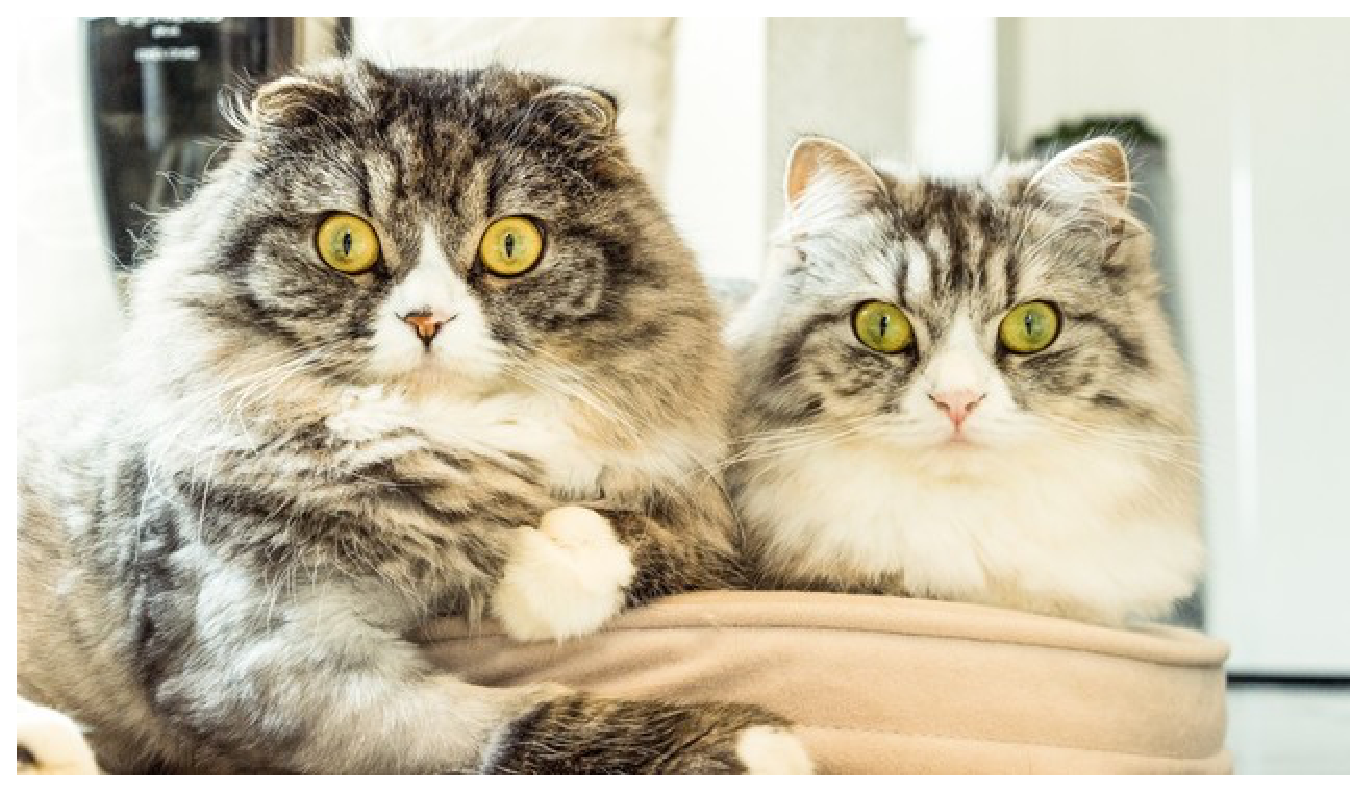
\includegraphics[width=8cm,clip]{assets/fig1.eps}
        \caption{Title of figure}
      \end{figure}
\end{frame}

\subsection{提案手法}
\begin{frame}{提案手法}
    \begin{align*}
        f(\mathbf{w}, b) =
            \highlightcap[red]{$\displaystyle \sum_{i=1}^k \left(y_i - \mathbf{w}^\top \mathbf{x}_i - b \right)^2$}{経験誤差}
            +
            \highlightcap[blue]{$\displaystyle \frac{\lambda}{2} \left\|\mathbf{w} \right\|^2$}{正則化項}
    \end{align*}
\end{frame}

\section{Evaluation}
\begin{frame}{評価方法・優位性}
    \begin{block}{Matrix Multiplication}
        \begin{algorithmic}[1]
            \STATE $C = O$
            \FOR{$i = 1, \dots, m$}
            \FOR{$j = 1, \dots, n$}
            \FOR{$k = 1, \dots, r$}
            \STATE $C[i,j] = C[i,j] + A[i, k] \cdot B[k, j]$
            \ENDFOR
            \ENDFOR
            \ENDFOR
            \RETURN $C$
        \end{algorithmic}
    \end{block}
\end{frame}

\section{Conclusion}
\begin{frame}{結論・貢献}
    \begin{columns}[t]
        \begin{column}{0.5\textwidth} % Split 50% and 50%
            \begin{figure}[htb]
              \centering
              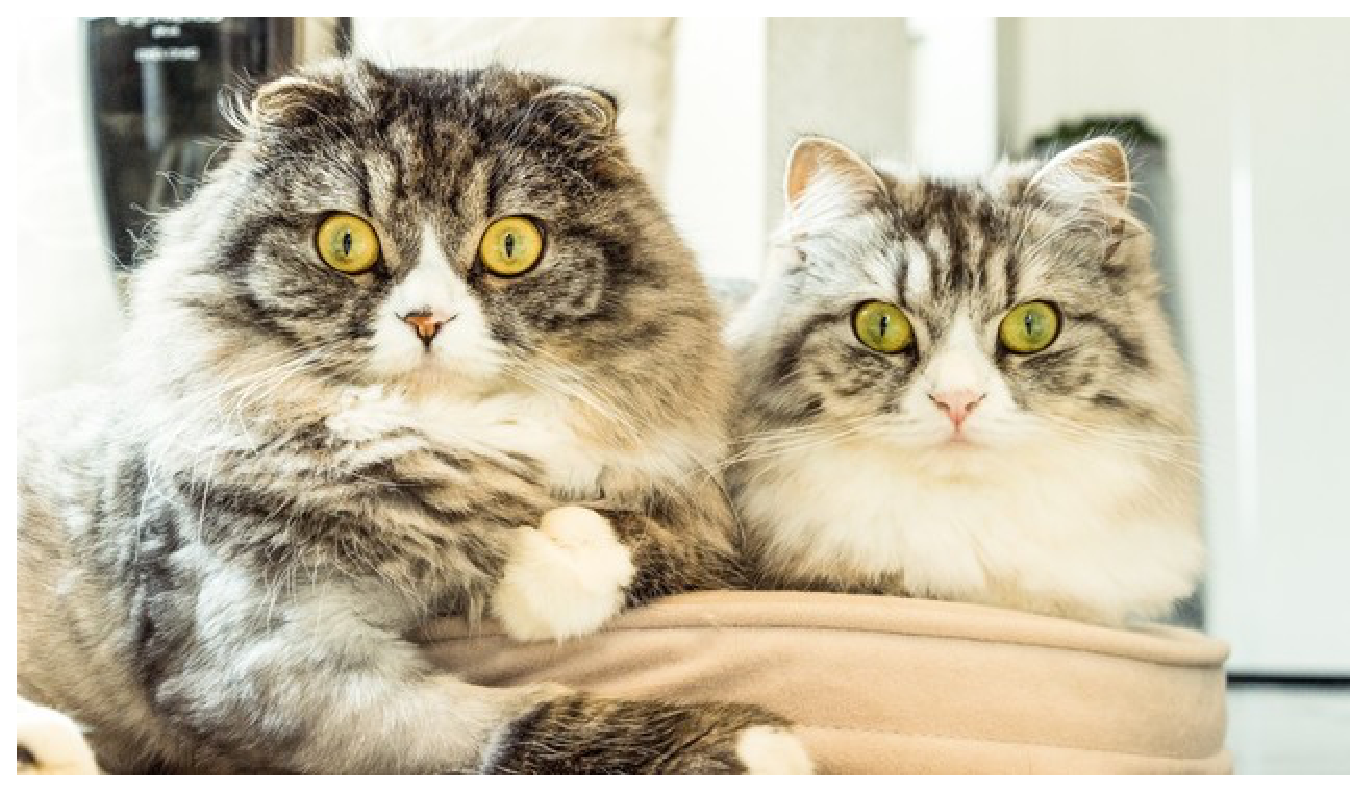
\includegraphics[width=3.5cm,clip]{assets/fig1.eps}
              \caption{Title of figure}
            \end{figure}%
        \end{column}
        \begin{column}{0.5\textwidth}
            \begin{figure}[htb]
              \centering
              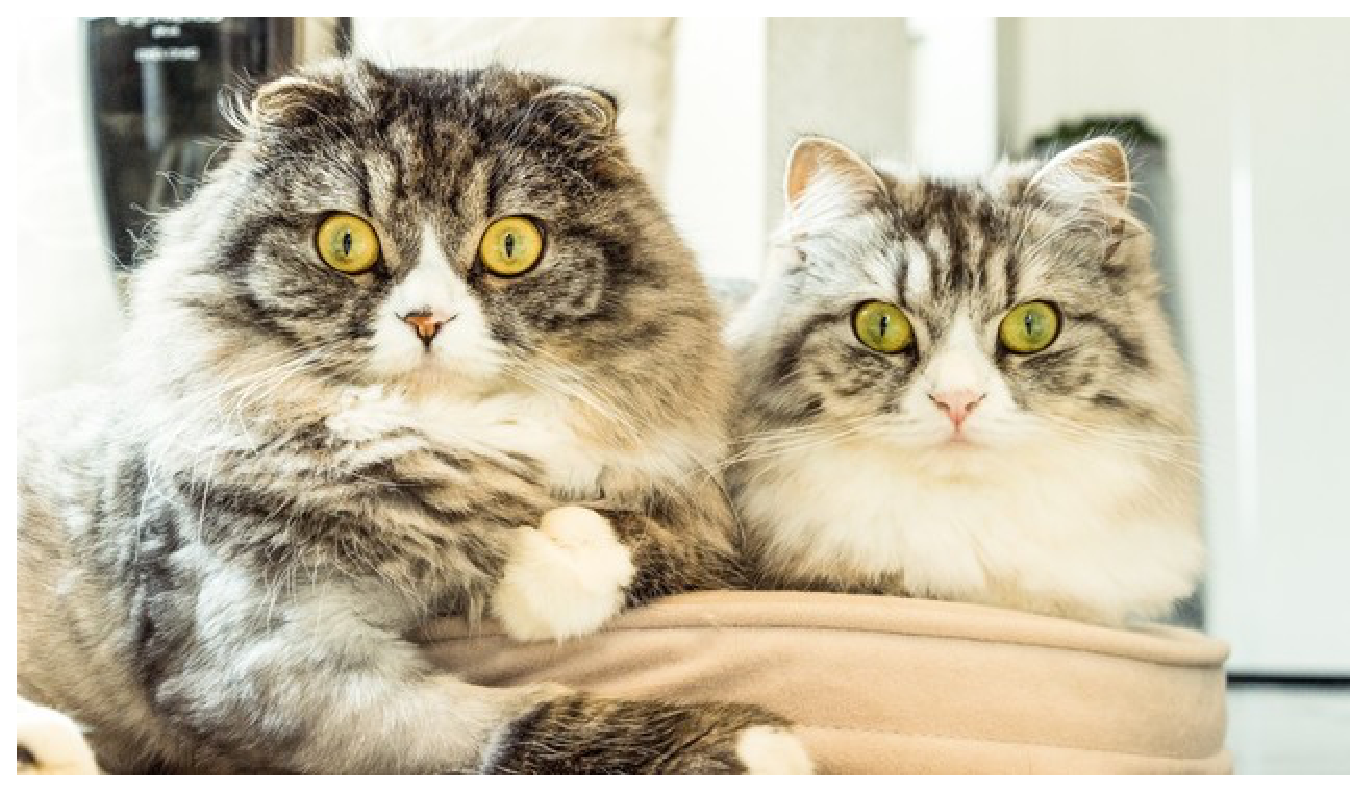
\includegraphics[width=3.5cm,clip]{assets/fig1.eps}
              \caption{Title of figure}
            \end{figure}%
        \end{column}
    \end{columns}
\end{frame}

\end{document}
